\documentclass[a4paper,10pt]{article}

\usepackage[english]{babel}
\usepackage{graphicx}
\usepackage[colorlinks, allcolors=black]{hyperref}
\usepackage{geometry}
\geometry{tmargin=3cm, bmargin=2.2cm, lmargin=2.2cm, rmargin=2cm}
\usepackage[colorinlistoftodos,prependcaption,textsize=small]{todonotes} %Used for the figure placeholder
\usepackage{minted}
\usepackage{color}
\usepackage{epstopdf}
\usepackage{lscape}
\usepackage{multirow}
\usepackage{subcaption}
\usepackage{amsmath}

\graphicspath{{../figures/}}

\begin{document}
\input{titlepage}
\tableofcontents

\section{Introduction}

\clearpage
\section{Active Shape Model}
In order to segment the incisors, an active shape model is built based on the provided training landmarks. A model is constructed for each individual incisor, resulting in eight models. This method is preferred over constructing one model for all incisors, because this would increase the variance of the landmarks.

To build this model, all the landmarks must be aligned. This is achieved by Procrustes analysis. A principal component analysis is performed on the aligned segmentations in order to analyse the variations of the segmentations, reduce the dimensionality and thus the complexity of the active shape model.
\subsection{Procrustes analysis}
The Procrustes analysis is done by taking the first segmentation sample and normalizing this sample. The other training examples are then optimally translated, scaled and then rotated to reduce the error between the corresponding landmark points. In the next iterations the reference sample is the mean of all the aligned segmentations. If the mean has converged, the process stops.

The optimal alignment is found by solving the weighted least squares problem, where the weights are based on the variance of the landmark points. High variance of a landmark means that the landmark is taken less into account in the error.

The result of the analysis is shown in figure \ref{fig:procrustes_single_tooth}.

\begin{figure}[htbp]
	\centering
	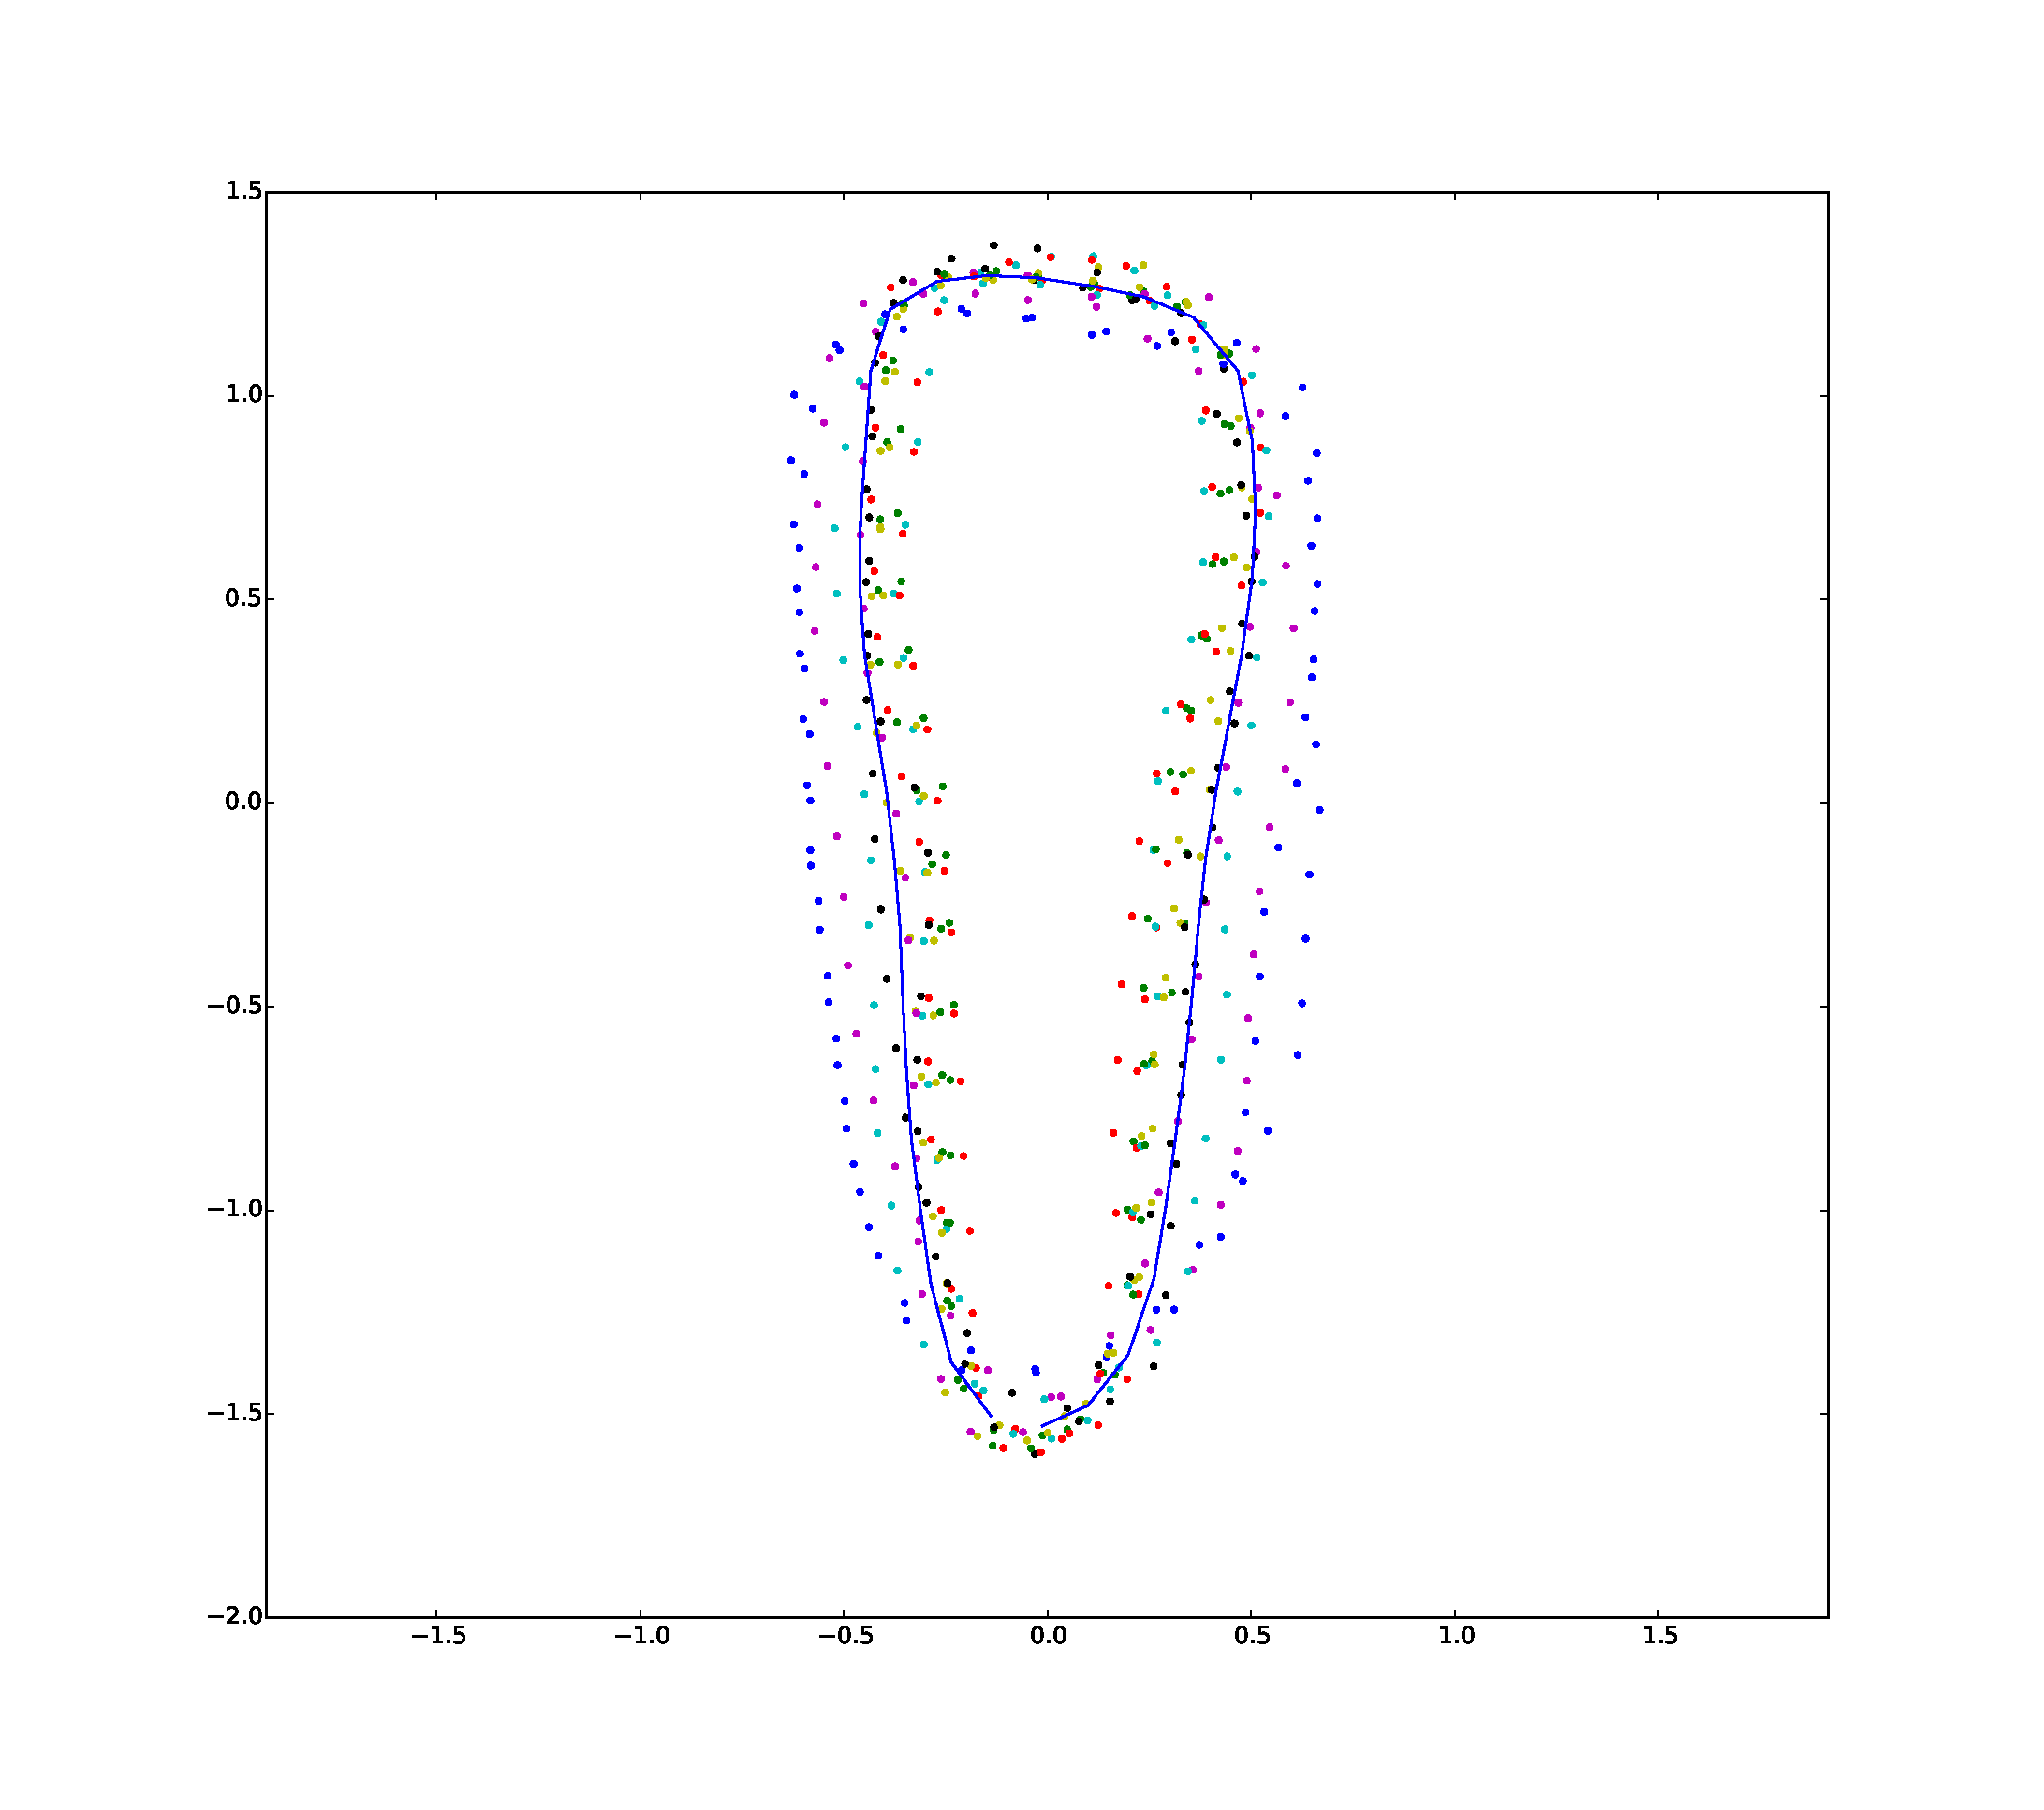
\includegraphics[width=0.9\textwidth, trim=0cm 2.5cm 0cm 3cm, clip]{procrustes_single_tooth}
	\caption{Alignment of training examples with the mean indicated for the third incisor}
	\label{fig:procrustes_single_tooth}
\end{figure}

\subsection{Principal component analysis}
The main objective of a principal component analysis is to reduce the dimensionality by representing the variables by principal components. These components are linear combinations of the variables. In order to keep as much information as possible, the components are chosen which explain the most variance. These components are the eigenvectors of the matrix containing the landmarks for the different images for one incisor. The eigenvectors corresponding to the highest eigenvalue explains the most of the variance. We chose to include the three first principal components for every incisor as these always explained between 80\% and 95\% of the variance. Notice that the 40 variables can be efficiently be reduced to three components.

The principal components can be seen in figure \ref{fig:pca_components}. The information explained by the principal components can be interpreted from these figures. The first principal component explains the width of the tooth, the second component explains the skewness of the tooth and the third component explains the ratio between the width of the top and bottom of the tooth. These interpretations hold for every model.

\begin{figure}[htbp]
	\centering
	\begin{subfigure}{0.30\textwidth}
		\centering
		\includegraphics[width=\textwidth, trim=0cm 2.5cm 0cm 3cm, clip]{pca1_pos}
		\caption{Positive value for the first PCA component}
	\end{subfigure}
	~
	\begin{subfigure}{0.30\textwidth}
		\centering
		\includegraphics[width=\textwidth, trim=0cm 2.5cm 0cm 3cm, clip]{pca2_pos}
		\caption{Positive value for the second PCA component}
	\end{subfigure}
	~
	\begin{subfigure}{0.30\textwidth}
		\centering
		\includegraphics[width=\textwidth, trim=0cm 2.5cm 0cm 3cm, clip]{pca3_pos}
		\caption{Positive value for the third PCA component}
	\end{subfigure}
	\\
	\begin{subfigure}{0.30\textwidth}
		\centering
		\includegraphics[width=\textwidth, trim=0cm 2.5cm 0cm 3cm, clip]{pca1_neg}
		\caption{Negative value for the first PCA component}
	\end{subfigure}
	~
	\begin{subfigure}{0.30\textwidth}
		\centering
		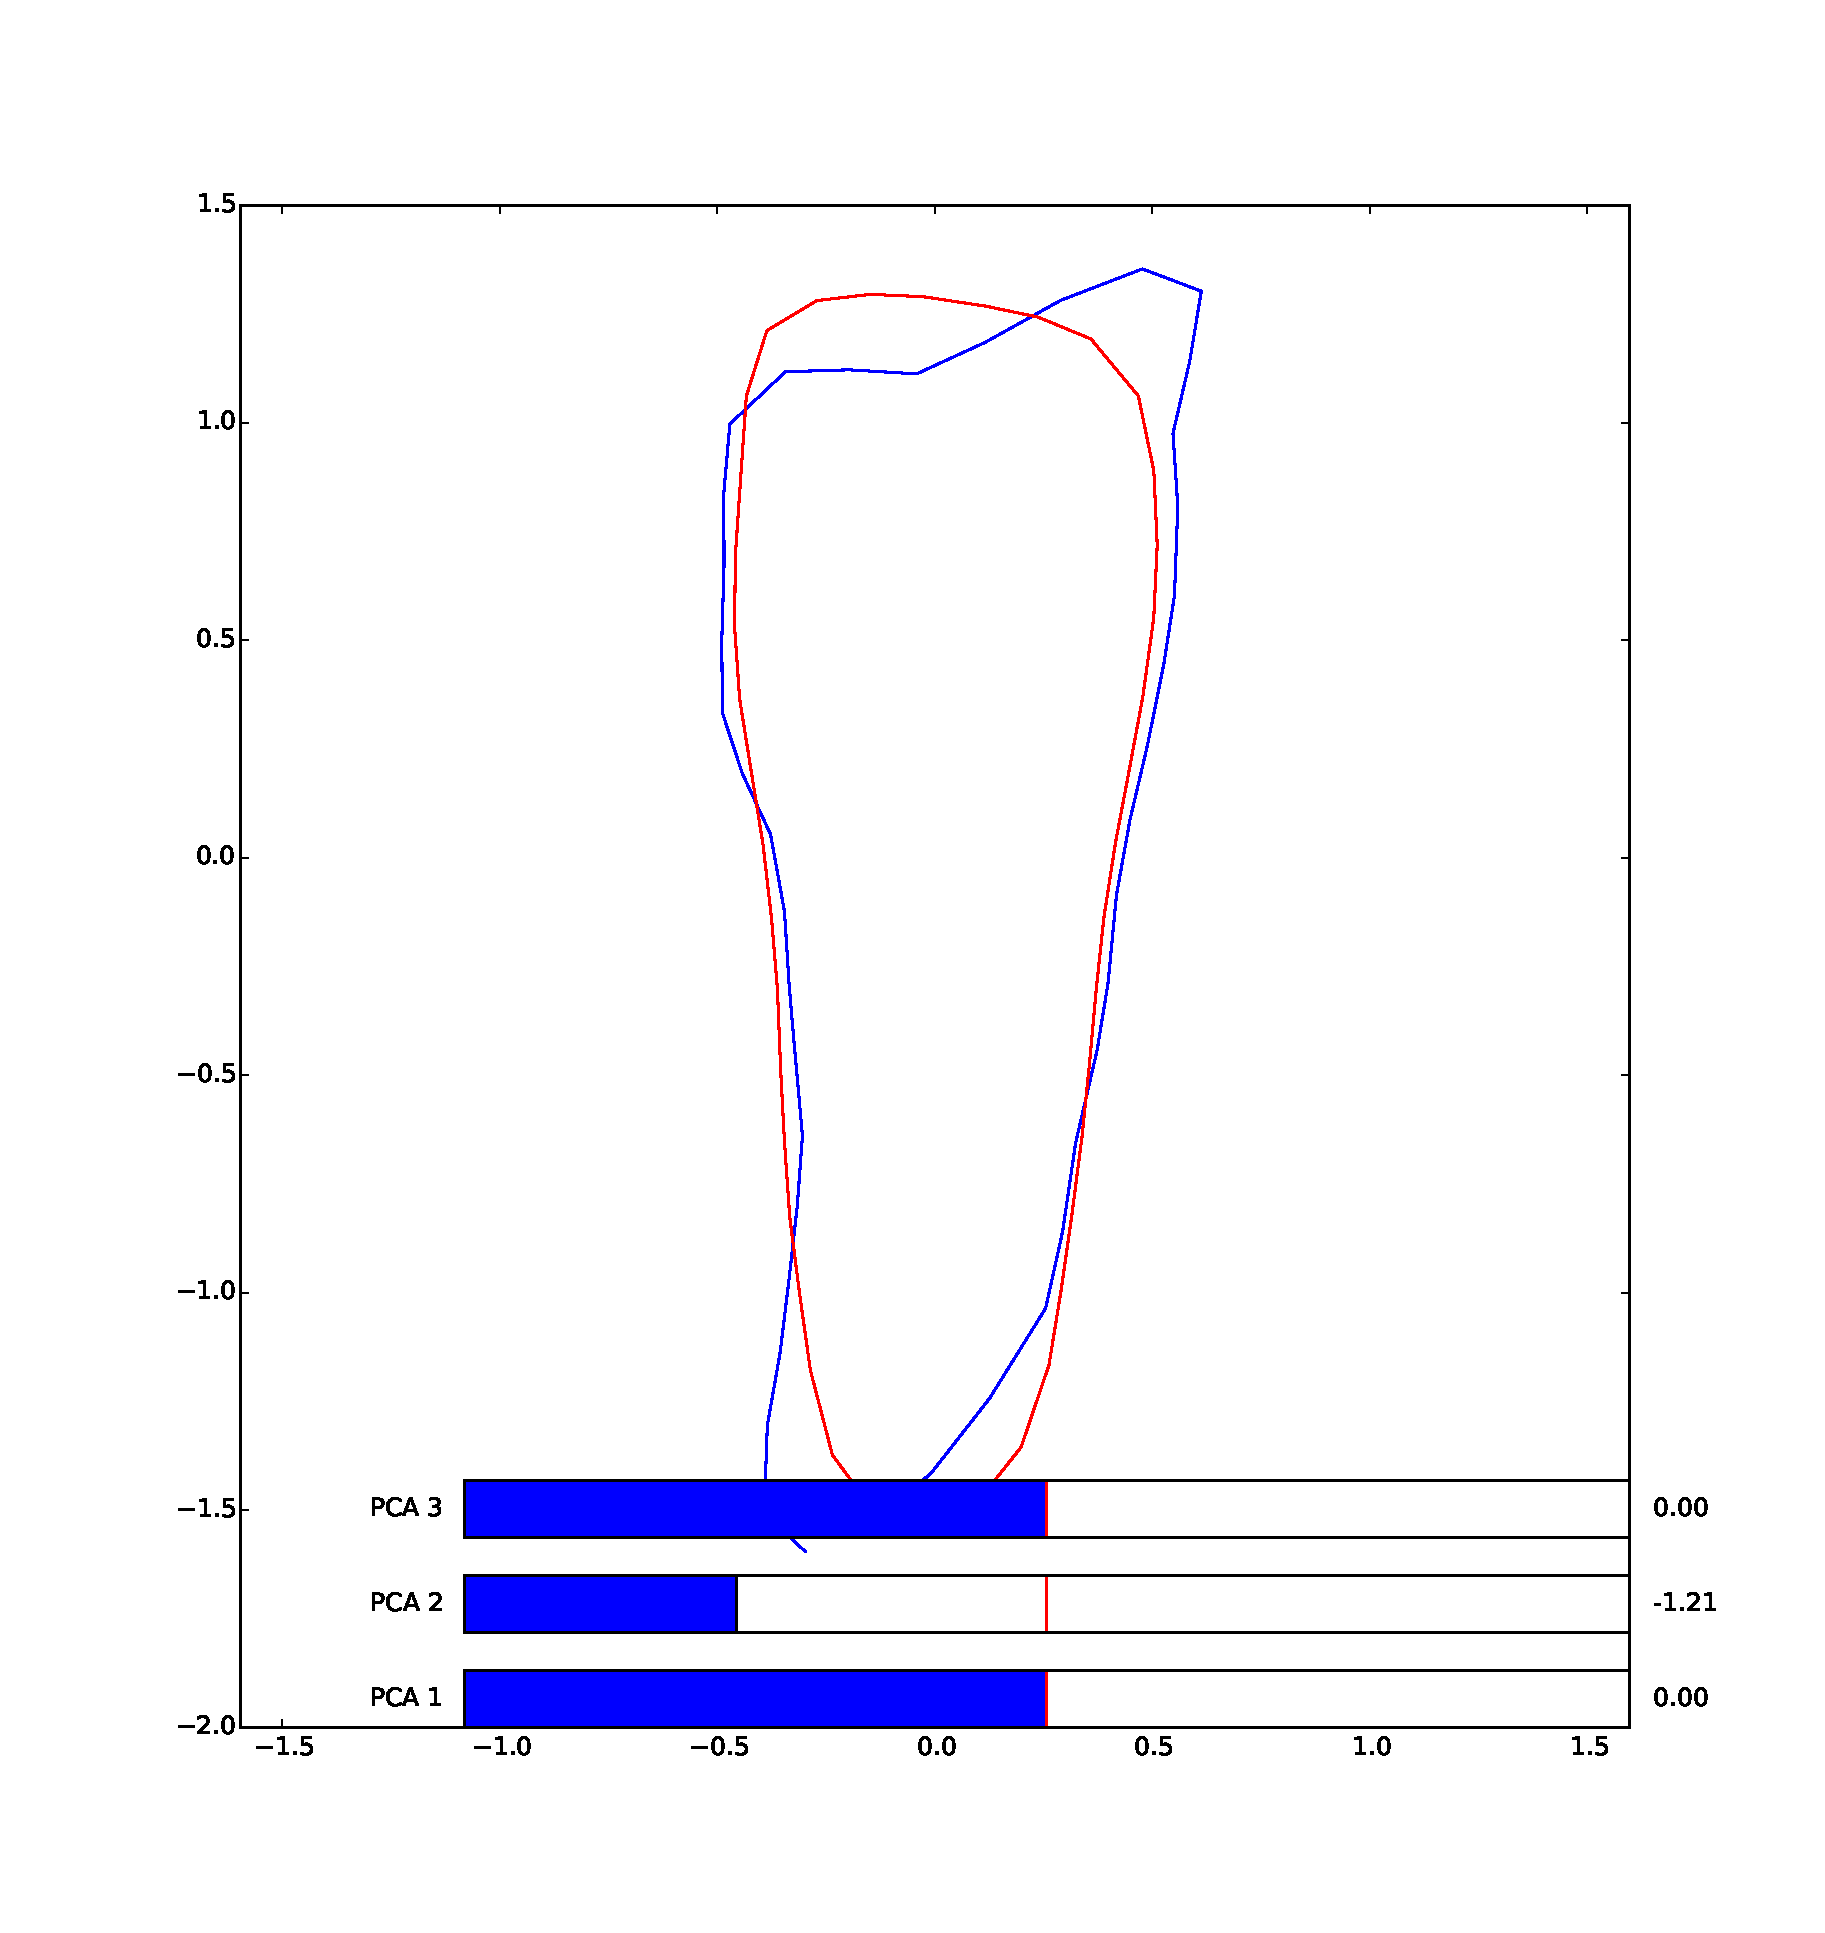
\includegraphics[width=\textwidth, trim=0cm 2.5cm 0cm 3cm, clip]{pca2_neg}
		\caption{Negative value for the second PCA component}
	\end{subfigure}
	~
	\begin{subfigure}{0.30\textwidth}
		\centering
		\includegraphics[width=\textwidth, trim=0cm 2.5cm 0cm 3cm, clip]{pca3_neg}
		\caption{Negative value for the third PCA component}
	\end{subfigure}
	\caption{PCA components; the mean model (red), adjusted model (blue)}
	\label{fig:pca_components}
\end{figure}

An approximation of the given segmentations by the model can be seen in figure \ref{fig:pca_tooth}. The exact landmarks of the tooth are plotted in green whereas the approximation is plotted in blue. This approximation is constructed by solving the following equation to find the parameter $b$:

\begin{equation*}
	x = \bar{x} + Pb
\end{equation*}

In this equation $\bar{x}$ is the mean model, $P$ is the projection matrix, containing the principal components and $x$ is the exact landmarks of the tooth. $b$ is thus a weighting for each principal component, these values are shown in the bottom right in figure \ref{fig:pca_tooth}.


\begin{figure}[htbp]
	\centering
	\includegraphics[width=0.9\textwidth, trim=0cm 2.5cm 0cm 3cm, clip]{pca_tooth}
	\caption{Approximation (blue) of a tooth (green) for the third active shape model (red)}
	\label{fig:pca_tooth}
\end{figure}


\section{Segmentation of the dental radiographs}
The goal of segmentation of the dental radiographs is to find bounding boxes around different teeth. To achieve this the radiographs are first pre-processed. After this the gap valley of the denture is located. The next step would be to find the vertical gaps between the teeth. This last step wasn't accomplished. Manual bounding boxes were drawn to test further parts of the algorithm.
\subsection{Pre-processing}
The goal of this step is to highlight the dark parts in the gap valley to ease the searching for the gap valley. The two most important steps in this pre-processing are iterative and adaptive thresholding. Iterative thresholding tries to find an intensity threshold to distinguish teeth from other areas in the radiograph. As to not remove any parts of the teeth it is preferred to only remove the areas of which we are absolutely sure that they are not teeth. The result of this thresholding can be seen in figure \ref{fig:it_thresh}. Notice that the gap and some places between the teeth are partly black. The initial threshold value for iterative thresholding is based on the average intensity near edges. Canny is used to find these edges. We assume that the most distinct edges correspond to teeth separations. The edges are dilated to find a better approximation for the initial thresholding value.

The last step is adaptive thresholding. Because the intensity of the radiograph varies in the image, a global thresholding does not perform good. Thresholding based on the intensity of the neighbourhood is accomplished by using adaptive thresholding. The results after iterative thresholding and adaptive thresholding can be seen in figure \ref{fig:result}. It can be seen that the gap valley is completely black.

\begin{figure}[htbp]
	\centering
	\begin{subfigure}{0.45\textwidth}
		\centering
		\includegraphics[width=\textwidth, trim=20cm 5cm 20cm 10cm, clip]{dilate}
		\caption{Blur + Canny + dilate}
		\label{fig:dilate}
	\end{subfigure}
	~
	\begin{subfigure}{0.45\textwidth}
		\centering
		\includegraphics[width=\textwidth, trim=20cm 5cm 20cm 10cm, clip]{it_thresh}
		\caption{Iterative thresholding}
		\label{fig:it_thresh}
	\end{subfigure}
	\\
	\begin{subfigure}{0.45\textwidth}
		\centering
		\includegraphics[width=\textwidth, trim=20cm 5cm 20cm 10cm, clip]{ad_thresh}
		\caption{Adaptive thresholding mask}
		\label{fig:ad_thresh}
	\end{subfigure}
	~
	\begin{subfigure}{0.45\textwidth}
		\centering
		\includegraphics[width=\textwidth, trim=20cm 5cm 20cm 10cm, clip]{result}
		\caption{Pre-processing result}
		\label{fig:result}
	\end{subfigure}
	\caption{Pre-processing steps (only a part of each image is shown)}
	\label{fig:pre_processing}
\end{figure}

\subsection{Gap valley detection}
Before searching for the gap valley a Gaussian filter is applied in the horizontal direction over inverse of the pre-processed image. The idea behind this is that it is more important to find a good gap in the middle of the image, close to the incisors. In figure \ref{fig:paths} the effect of this filter can be seen.

To find the gap valley intensity histograms are calculated at intervals over the width of the image. The intensities are the sum of the intensities lying in a horizontal range at each height. A plot of these intensities is shown in figure \ref{fig:fourier}. This histogram is then smoothed using a Fourier transformation. The maxima in this histogram represent points in the image through which the optimal path might pass. For each interval the four best points are kept as candidates. In the next step paths are generated between these points to find the optimal path. For each point an edge is added to the point with the lowest increase in intensity. The created paths are then trimmed and pruned based on their remaining length. The cost of the path is equal to the intensity of all points on this path in the original pre-processed image.

\begin{figure}[htbp]
	\centering
	\includegraphics[width=0.9\textwidth, trim=0cm 2.5cm 0cm 3cm, clip]{fourier_intensity}
	\caption{Fourier transformation of intensity histogram for one vertical slice of the image \\(pixel index on x-axis, intensity on y-axis)}
	\label{fig:fourier}
\end{figure}

\begin{figure}[htbp]
	\centering
	\includegraphics[width=1\textwidth, trim=0cm 0cm 0cm 0cm, clip]{paths}
	\caption{The remaining horizontal paths after pruning (blue) and the horizontal path for the gap valley (yellow), with the line intensity on the pre-processed image}
	\label{fig:paths}
\end{figure}


\section{Fit the model to an image}
\subsection{Initial fit}

\subsection{Update pose and shape parameters to fit model to image landmarks}

\subsection{Find landmarks on image based on neighbourhood near model points}

\subsection{Multi-resolution fitting}


\section{Evaluation}


\todo[inline]{Bronnen}
\end{document}
